\section{正定函数(能量函数)}\label{2Bref}
\begin{definition}[正定、正半定、负定、负半定函数]
  称一函数$V:D\to\R$是\begin{itemize}[leftmargin=1em]
    \item {\bf 正定的(positive definite)},若$V(0)=0$且对任意$x\ne 0$均有$V(x)>0$;\index{正定(positive definite)}
    \item {\bf 正半定的(positive semidefinite)},若$V(0)=0$且对任意$x\ne 0$均有$V(x)\ge0$;\index{正半定(positive semidefinite)}
    \item {\bf 负定的(negative definite)}/{\bf 负半定的(negative semidefinite)},若$-V(x)$是正定/正半定的。\index{负定的(negative definite)}\index{负半定的(negative semidefinite)}
  \end{itemize}
\end{definition}
\begin{note}
  需要特别注意,上面这些函数的输出均为标量,且在$0$处取值均为$0$。
\end{note}
\begin{example}[正定、正半定函数]
  令$x=(x_1,x_2)^\mathrm{T}$。那么
  \begin{itemize}[leftmargin=1em]
    \item $V(x)=x_1^2$是正半定的,因为其在原点处取值为$0$,对于所有$x$均为非负,且对所有满足$x_1=0$($x_2$可为任意值)的$x$均等于$0$。
    \item $V(x)=x_1^2+x_2^2$是正定的,因为其在(且仅在)原点处取值为$0$,对于所有$x$均为非负。
    \item $V(x)=x_1^2+x_2^2+1$不符合正定的定义,因为其在原点处取值不为$0$。
    \item $V(x)=\frac{x_1^2}{1+x_1^2}+x_2^2$是正定的,理由同第二例。
    \item $V(x)=(x_1^2,x_2^2)^\mathrm{T}$不符合正定的定义,因为它的输出不是标量。
  \end{itemize}
\end{example}

\begin{example}[局部正定函数]
  考虑$V(x)=x^2(4-x^2)$($x$为标量),若规定$x\in(-2,2)$,则该函数是正定的;若$x\in[-2,2]$,则该函数是正半定的;对于其余情形,原函数不定。
\end{example}

下面以一个物理系统说明正定函数的物理含义。
\begin{example}[正定函数与能量]\label{pendulum}
  考虑右图所示的含阻尼单摆系统,根据物理知识可写出其动力学方程(注意阻力与速度$l\dot{\theta}$成正比且反向)
  \[lm\ddot{\theta}=-kl\dot{\theta}-mg\sin\theta\]

  \begin{wrapfigure}{R}{0.18\textwidth}
  	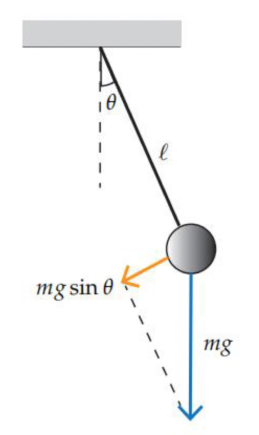
\includegraphics[width=\linewidth]{./figure/nonlinear/pendulum.png}
    \captionof{figure}{带阻尼单摆系统}
  \end{wrapfigure}

  定义$x=(\theta,\dot{\theta})^\mathrm{T}$(限制$-\pi<\theta\le \pi$),那么可写出其状态空间表达式
  \begin{align*}
    \dot{x}_1&=x_2\\
    \dot{x}_2&=-\frac{k}{m}x_2-\frac{g}{l}\sin x_1
  \end{align*}
  
  根据物理中的动能和势能(选最低点为零势能面),写出其总能量\begin{align*}
    V&=\frac{1}{2}mv^2+mgh\\
    &=\frac{1}{2}m(l\dot{\theta})^2+mgl(1-\cos\theta)\\
    &=\frac{1}{2}m(lx_2)^2+mgl(1-\cos x_1)
  \end{align*}

  可见$V$是正定的。求其对$t$的导数可得\begin{align*}
    \dot{V}&=ml^2x_2\dot{x}_2+mgl(\sin x_1)\dot{x}_1\\
    &=ml^2x_2\left(-\frac{k}{m}x_2-\frac{g}{l}\sin x_1\right)+mgl(\sin x_1)x_2\\
    &=-kl^2x_2^2\le0
  \end{align*}

  可见$\dot{V}$是负半定的,意即系统的能量随时间而衰减——这同系统有阻尼相合。
  本例说明,正定函数可看作对于系统内存储的“能量”的数学抽象。之后我们会看到,所有的Lyapunov稳定性定理
  都聚焦于沿系统状态变动的正定函数及其随时间的导数。
\end{example}

最简单也是最为常见的正定函数是{\bf 二次型(quadratic form)}\index{二次型(quadratic form)},其为自$\R{}^n$至$\R{}$的函数\[V(x)=x^\mathrm{T}Px\]其中$P=P^\mathrm{T}\in\R{}^{n\times n}$。二次型函数$V(x)$的正定/正半定/负定/负半定性,取决于$P$的正定/正半定/负定/负半定性。
下面定理证明略去,可参看本科线性代数教材。
\begin{theorem}[实对称矩阵正定、正半定、负定、负半定的判据]\label{pd_nd_thm}
  矩阵$P=P^\mathrm{T}\in\R{}^{n\times n}$是\begin{itemize}[leftmargin=1em]
    \item 正定的,当且仅当其全部特征值都为正,或其所有顺序主子式(矩阵的$i$阶顺序主子式,系矩阵的前$i$行前$i$列这一子块的行列式)均为正;
    \item 正半定的,当且仅当其全部特征值都非负,或其所有主子式(矩阵的$i$阶主子式,系选取$i$行,再以这些行的行号作为列号,取出这些行中对应列的元素,再按原方位排列所构成的$i$阶行列式)均为非负;
    \item 负定的,当且仅当其全部特征值都为负,或其奇数阶顺序主子式为负,偶数阶顺序主子式为正。
    \item 负半定的,当且仅当其全部特征值都非正,或其所有主子式均为非正。
  \end{itemize}
\end{theorem}
\begin{definition}[相似与合同]
  \begin{itemize}[leftmargin=1em]
    \item 称两矩阵$A,B$相似,若存在可逆阵$S$使得$S^{-1}AS=B$;
    \item 称两矩阵$A,B$合同,若存在可逆阵$S$使得$S^{\mathrm{T}}AS=B$。
  \end{itemize}
\end{definition}
\begin{theorem}[实对称矩阵的正交相似对角化]\label{ortho_sim_diag}
  对于任意$P=P^\mathrm{T}\in\R{}^{n\times n}$,均存在一正交矩阵$U$(即$U^\mathrm{T}U=I$)使得$U^{-1}PU=\Lambda$(也即$U^{\mathrm{T}}PU=\Lambda$),
  其中$\Lambda$为对角矩阵,且其对角线上的元素为$P$的所有特征值(均为实数,各特征值出现次数等于代数重数)。
\end{theorem}
注意下述定理无需附加实对称的前提,因为$C^\mathrm{T}C$一定是对称的。
\begin{theorem}[正定、正半定矩阵的分解]\label{pd_npd_div}
  矩阵$P\in\R{}^{n\times n}$是正半定的,当且仅当存在一矩阵$C\in\R{}^{n\times n}$,使得$P=C^\mathrm{T}C$;
  进一步地,$P$是正定的当且仅当$C$可逆(或称为合同于单位阵)。进而,正定矩阵彼此合同。
\end{theorem}
\begin{theorem}[Rayleigh-Ritz不等式]\label{rayleigh-ritz}
  设$P=P^{\mathrm{T}}\in\mathbb{R}^{n\times n}$,并设$\lambda_\mathrm{max}$和$\lambda_\mathrm{min}$分别是$P$的最大特征值和最小特征值。则有
\[\lambda_{\mathrm{min}}\|x\|_{2}^{2}\le x^{\mathrm{T}}Px\le \lambda_{\mathrm{max}}\|x\|_{2}^{2}\]
\end{theorem}
证明可见\href{https://oliverwu.top/file/rayleigh-ritz.pdf}{链接}。